%fichier : Projet_Di4_PPGL_Chana_Pecault.tex
%Date : 21/09/2021
%Version : 1.00
%Modif : 21/09/2021

\documentclass{EPUProjetDi}
\usepackage[bottom]{footmisc}
\usepackage{txfonts}
\usepackage{float}
\makeindex

%remplir les lignes suivantes avec les informations vous concernant :
\title[Simulation d'une colonie de fourmis]{Simulation d'une colonie de fourmis}

\projet{Projet de Programmation et Génie Logiciel}

\author{
Narvin Chana\\ %Attention : toujours écrire d'abord le prénom puis le nom (ne pas mettre tout le nom en majuscules)
\noindent[\url{narvin.chana@etu.univ-tours.fr}]\\
Noé Pécault\\ %Attention : toujours écrire d'abord le prénom puis le nom (ne pas mettre tout le nom en majuscules)
\noindent[\url{noe.pecault@etu.univ-tours.fr}]}

\encadrant{Nicolas Monmarché\\ %
\noindent[\url{nicolas.monmarche@univ-tours.fr}]\\~\\
Polytech Tours\\
Département Informatique\\~ %
}

%%%%%%%%%%%%%%%%%%%%%%%%%%%%%%%%%%%%%%%%%%%%%%%%%%%%%%%%%%%%%%%%%%%%%%%%%%%%%%%%%%%%%%%%%%
\begin{document}

\maketitle

\pagenumbering{roman}
\setcounter{page}{0}

{
%on réduit momentanément l'écart entre paragraphes pour ne pas trop aérer la table des matières
\setlength{\parskip}{0em}

\tableofcontents

%\listoffigures
%rq1 : si vous n'avez pratiquement pas de figures, laissez la ligne précédente en commentaire

%\listoftables
%rq1 : si vous n'avez pratiquement pas de tables, laissez la ligne précédente en commentaire
}


\start
%%%%%%%%%%%%%%%%%%%%%%%%%%%%%%%%%%%%%%%%%%%%%%%%%%%%%%%%%%%%%%%%%%%%%%%%%%%%%%%%%%%%%%%%%%

\chapter*{Introduction}
%le 2 lignes suivantes permettent d'ajouter l'introduction à la table des matières
%et d'afficher "Introduction en haut des pages"
\addcontentsline{toc}{chapter}{\numberline{}Introduction}
\markboth{\hspace{0.5cm}Introduction}{}

\paragraph{}
Le problème de la simulation et de l'optimisation d'une colonie de fourmis est un problème complexe 
qui met en \oe{}uvre des connaissances dans les domaines de la théorie des graphes, la recherche opérationnelle 
et dans les systèmes décentralisés. Chaque fourmi agit par elle-même et l'ensemble des fourmis forme une intelligence
à part entière qui n'a pas de cerveau centralisé.

Ses applications sont vastes et interviennent dans des domaines tels que les problèmes d'ordonnancements, 
de routage (Ex : réseau Internet ou tournée de véhicules) ou encore le traitement d'image (Ex : détection de bords).

Ce problème de simulation de colonie de fourmis nous intéresse depuis longtemps et c'est donc pour cela que dans 
le cadre du projet de programmation et génie logiciel, nous avons choisi de proposer un sujet qui traite de celui-ci.

Notre objectif pour ce projet était de créer une application permettant de simuler les interactions qu'une colonie 
de fourmis peut avoir avec son environnement. Les fourmis doivent pouvoir explorer les alentours de leur colonie afin 
de trouver de la nourriture et de la ramener à sa colonie. 
Nous avions aussi imaginé d'autres fonctionnalités qui pourraient venir se greffer au projet si le temps nous le permettait
comme des combats entre fourmilières et la possibilité de simuler plusieurs colonies.

En revanche, il n'était pas dans nos objectifs de simuler l'intérieur de la colonie et la simulation n'est pas voué à être sur le long terme
(nous ne prenions donc pas en compte la durée de vie des fourmis).

Il nous était également très important de respecter les principes de génie logiciel qui nous ont été appris durant notre
parcours à Polytech dans le but de développer une application robuste et facilement extensible.

Au sein de ce rapport, nous présenterons notre démarche pour arriver aux objectifs fixés, le déroulement du projet ainsi que les résultats, 
et ce dont on en a tiré.

\chapter{Conception et décisions}

Ce chapitre traite des objectifs et contraintes du projet, de son architecture et des interactions entre les différents modules. 
Nous y détaillons aussi les différentes entités et structures qui appartiennent à la simulation ainsi que la structure de la partie applicative.

\section{Objectifs et contraintes}

\subsection*{Système décentralisé}

Un système décentralisé \footnote[1]{Page wikipedia : \url{https://en.wikipedia.org/wiki/Decentralised_system}} est un système composé de sous-composants qui accomplissent des objectifs individuellement afin
de réussir un objectif global.
Les entités qui composent le système doivent interagir entre elles non pas via une intelligence globale, mais par des moyens de communication plus locaux.

Le problème de la simulation de colonie est une application typique de ce principe et se retrouve même dans la nature.
Dans une vraie fourmilière, il n'y a aucune entité qui donne les ordres aux autres et donc chaque fourmi connaît sa mission
pour faire prospérer la colonie. 

Il est donc essentiel pour notre simulation de respecter cette architecture et chaque fourmi doit donc prendre ses décisions
avec seulement les informations qui lui sont accessibles.

\subsection*{Simulation personnalisable}

La simulation doit aussi être un outil facile à utiliser afin de tester des configurations initiales différentes.
Il en va de même pour les constantes de simulation comme la portée de perception des fourmis, leur vitesse et toutes les autres.

Nous cherchons donc à avoir une interface graphique simple à utiliser qui permettra de placer les éléments de la simulation à la guise
de l'utilisateur.

\subsection*{Séparation Moteur et Application}

Une des contraintes clés du projet est la séparation de la partie \textbf{Moteur de simulation} et \textbf{Application}.
Cela permet de réutiliser ce moteur pour d'autres applications comme par exemple pour générer des trajectoires de fourmis 
pour une animation.

Cela nous contraint donc à faire en sorte que le moteur n'ait absolument aucune dépendance envers la partie application.

\subsection*{Abstraction des entités pour l'évolutivité}

Nous avons intérêt à garantir une certaine évolutivité de la simulation car le comportement des fourmis que nous avons conceptualisé
n'est pas forcément exact et nous devions nous permettre de facilement le changer.

Il est même aussi possible que nous souhaitions utiliser ce même moteur pour simuler des comportements autre que
des fourmis ce qui force un certain niveau d'abstraction.

\subsection*{Optimisation future}

La simulation de colonie de fourmis est un problème très gourmand en termes de ressources de calcul car il est nécessaire de calculer les mouvements
de chaque fourmi à une cadence assez élevée pour atteindre un taux de mise à jour par seconde proche suffisant pour que la simulation paraisse fluide 
(60 images par seconde).

Une piste d'optimisation dont nous avons eu conscience au moment de la conception est de paralléliser le calcul des fourmis tout en s'assurant de maintenir
l'intégrité des résultats de la simulation (pas de problème de concurrence).

Nous cherchons donc une architecture nous ouvrant la possibilité d'implémenter facilement une telle technique d'optimisation sans avoir à
refaire l'architecture de 0. 

\pagebreak

\section{Moteur}

\subsection{Structure générale}

Le moteur de simulation est donc là où les calculs de trajectoire et de décisions des fourmis seront effectués.
Sa structure est simple et est très largement inspirée de ce qu'on peut trouver dans le domaine du jeu vidéo et 
cela n'est pas étonnant, car notre simulation se rapporte beaucoup à un jeu vidéo.

Tout d'abord, les individus de notre simulation sont des \textbf{Entités}. Une entité est un objet associé à un
\textbf{Transform} qui représente un état physique dans le monde (position, rotation, taille) et aussi d'un comportement
qui lui est défini dans une méthode Update() sous la forme d'une suite d'instructions.

Cet objet Transform\footnote{Page du manuel d'Unity sur l'objet Transform \url{https://docs.unity3d.com/Manual/class-Transform.html}} 
est une inspiration directe du jeu vidéo et plus précisément du moteur de jeu Unity

On a l'objet qui sert de chef d'orchestre à la simulation qui est le \textbf{Monde}. Il possède les propriétés concernant 
l'environnement des fourmis et contient aussi la totalité des entités présentent dans la simulation.
Lorsqu'il est mis à jour, le monde doit donc mettre à jour la totalité des entités qu'il contient pour que chaque entité 
puisse exécuter ses actions.

Nous appelons la mise à jour de ce monde et des entités qui le compose, un \textbf{tick}.

\begin{figure}[h]
    \centering
    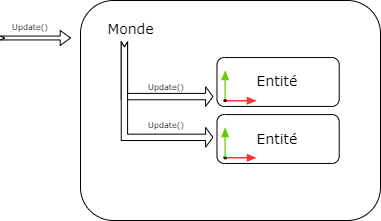
\includegraphics[scale=0.8]{moteur_structuregenerale.png}
    \caption{Flux de mise à jour}
    \label{fig:flow_update}
\end{figure}

\autoref{fig:flow_update} montre le processus de mise à jour de la simulation qui commence par le monde et 
qui est distribuée à toutes les entités qu'il contient.

\pagebreak
\subsection{Entités}

\subsubsection*{Définition}

Ce que nous appelons \textbf{Entité} est un objet possédant un état physique qui est composé d'une position, une rotation et une taille (\textbf{Transform}) 
ainsi que d'une logique interne que l'on appellera comportement.

Cette association de position, rotation et d'une taille est ce qu'on appelle un \textbf{Transform} et caractérise l'existence dans le monde de l'entité.
La définition de cet objet nous est utile car elle nous permet de manipuler l'état de l'entité dans une même structure et d'appliquer des transformations
linéaires simplement dans le cas où l'on voudrait faire un système de coordonnées relatif à une autre entité.

Les entités sont les briques essentielles à la simulation car elles représentent les objets de notre simulation. 

\subsubsection*{Spécialisations des entités}

La classe \textbf{Entity} est donc la version la plus abstraite d'un de ces objets et chacune de ses spécialisations
représentera une entité au comportement différent pouvant exister dans la simulation.

Les comportements ajoutés sont par exemple le système de vie, une machine à états ou même le comportement d'une fourmi.
Le dernier composant présent dans chaque entité est le \textbf{Collider} qui est la boîte de collision d'une entité et peut se définir 
de différentes formes selon les besoins. Il est utile dans le calcul des mouvements car il permet de tester si une entité ne cherche pas 
à se déplacer dans un mur.

\autoref{fig:struct_entities_spec} montre l'arborescence des entités avec ce que chacune apporte comme fonctionnalité.

\begin{figure}[h]
    \centering
    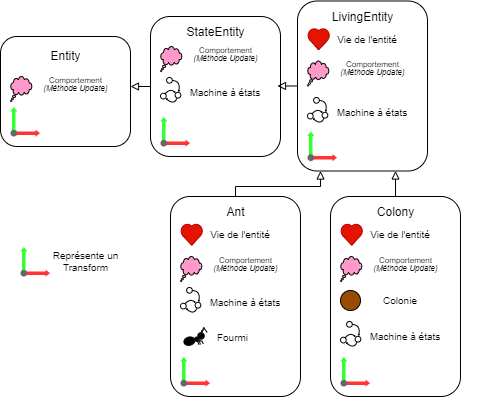
\includegraphics[scale=0.5]{entities_specialisations.png}
    \caption{Diagramme des spécialisations des entités avec leurs apports}
    \label{fig:struct_entities_spec}
\end{figure}

\subsection{World}

\subsubsection*{Définition}

Le monde est l'espace dans lequel la simulation se déroule et possède donc les propriétés de taille de la simulation ainsi que le Collider
gérant les murs de la simulation.
C'est lui qui stocke toutes les entités présentent dans la simulation et s'occupe de les mettre à jour lorsqu'il est lui-même mis à jour. 
(voir \autoref{fig:flow_update})

Par souci d'optimisation, le monde est divisé en régions qui sont chacune une liste des entités présentes dans la région. 
Cela permet de ne pas avoir à chercher des éléments parmi la liste complète de toutes les entités du monde.
Le monde est donc responsable du maintient de la cohérence de ces régions et met à jour toutes ces listes en fonction des positions
des entités à chaque instant T.

\begin{figure}[h]
    \centering
    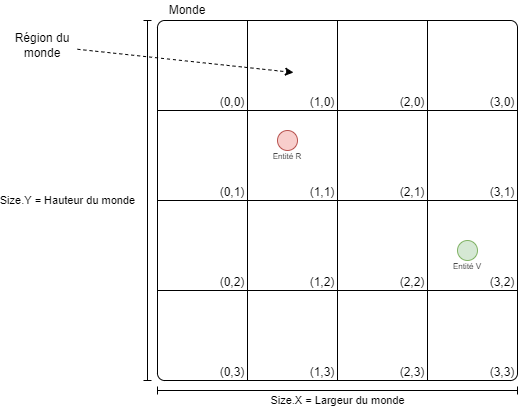
\includegraphics[scale=0.5]{world.png}
    \caption{Schéma d'un monde avec ses régions}
    \label{fig:world_scheme}
\end{figure}

Les murs de la simulation sont représentés par le WorldCollider qui est un second découpage (indépendant des régions) ayant pour but 
de stocker les cases traversables ou non par les autres entités.
Cette représentation des murs sous forme d'une matrice de booléens nous permet d'avoir une structure analogue à une image ayant pour chaque pixel
une valeur \textbf{Vrai} pour représenter un mur ou \textbf{Faux} pour représenter une case traversable.

\begin{figure}[h]
    \centering
    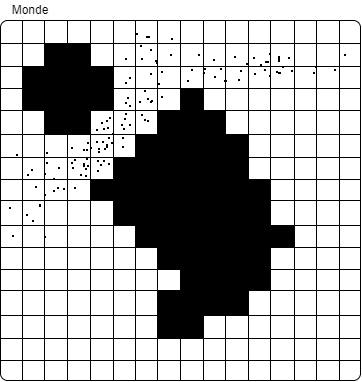
\includegraphics[scale=0.4]{world_collider.png}
    \caption{Schéma d'un monde avec ses murs }
    \label{fig:world_collider_scheme}
\end{figure}

\subsection{Colliders}

Pour notre simulation, nous avons prévu trois types de boîtes de collision différents. Ces types de collisions
peuvent tous les trois être testés entre eux afin de savoir si oui ou non ils sont superposés (s'ils sont en collision).

\subsubsection*{Cercle - Monde}

Dans la collision entre un cercle et un monde, on procède en trois étapes:
\begin{itemize}
    \item Créer un carré imaginaire dans lequel le cercle est inscrit.
    \item Récupérer le sous-ensemble des cases du WorldCollider que ce carré superpose.
    \item Tester si chaque case de ce sous-ensemble est superposée au cercle d'origine.
\end{itemize}

\begin{figure}[h]
    \centering
    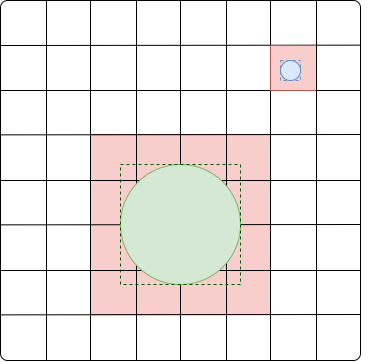
\includegraphics[scale=0.6]{world_collider_circle.png}
    \caption{Schéma de la collision d'un cercle et du monde}
    \label{fig:world_collider_circle}
\end{figure}

\pagebreak

\subsubsection*{Rectangle - Rectangle}
\paragraph{}
La collision entre un rectangle et un autre rectangle semble simple mais quand on rend possible la rotation de ces rectangles l'algorithme devient légèrement plus complexe.
Pour faire cela on utilise le \textbf{Separating Axis Theorem (SAT)}\footnote{} qui énonce le suivant :

\textit{Deux objets convexes ne se superposent pas s'il existe un axe sur lequel la projection des points de ces deux objets ne se superposent pas.}

L'avantage de ce théorème est qu'il est extrêmement rapide à s'executer (lorsqu'on voit qu'une projection sur un de leurs axes ne sont pas superposés on peut arrêter l'algorithme).
Voici quelques exemples pour illustrer : 

\begin{figure}[h]
    \centering
    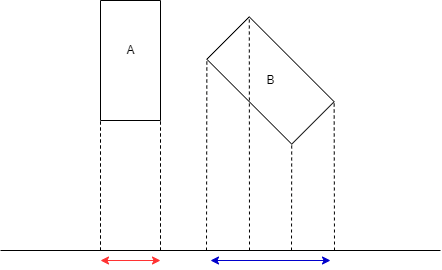
\includegraphics[scale=0.6]{rectangle_collider_rectangle_1.png}
    \caption{Schéma de deux rectangles qui ont une projection sur un de leurs axes qui collisionne pas.}
    \label{fig:rectangle_collider_rectangle_1}
\end{figure}

Dans la figure \ref{fig:rectangle_collider_rectangle_1}, on voit que les deux objets ne se superposent pas en raison de la non intersection des segments rouge et bleu.

\begin{figure}[h]
    \centering
    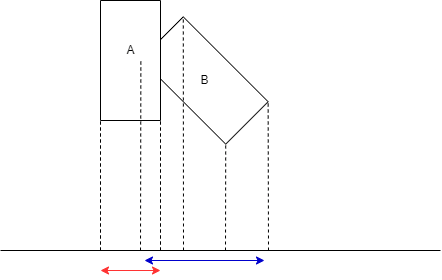
\includegraphics[scale=0.6]{rectangle_collider_rectangle_2.png}
    \caption{Schéma de deux rectangles qui ont une projection sur un de leurs axes qui collisionne.}
    \label{fig:rectangle_collider_rectangle_2}
\end{figure}

Dans la figure \ref{fig:rectangle_collider_rectangle_2}, on doit tester tous les autres axes des deux objets car les segments rouge et bleu se superposent.
Si toutes les projections collisionnent, alors, les deux objets se superposent.

\subsubsection*{Rectangle - Cercle}
La collision entre un rectangle et un cercle peut utiliser l'algorithme précédent et 
le cercle prendra en axe, la droite formée par le centre du cercle et le point du rectangle qui est la plus proche.

\subsection{Fourmis}

Dans cette partie nous allons détailler comment nous avons imaginé une représentation du comportement de la colonie, des fourmis et des phéromones.

\subsubsection{Comportement d'une fourmi}

L'objectif final de la fourmi est simple, elle veut trouver de la nourriture pour la ramener à sa colonie. Cependant, nous ne pouvons pas seulement
faire marcher la fourmi au hasard dans la simulation en espérant qu'elle atteigne ce but. 

Les fourmis sont indépendantes mais ont un objectif commun et doivent donc pouvoir communiquer entre elles pour parvenir à accomplir cet objectif.
Dans la vraie vie, le principe d'une fourmi est très complexe et varie énormément entre les espèces mais nous pouvons le vulgariser très simplement.

Une fourmi va partir de sa colonie à la recherche de nourriture tout en déposant des phéromones pour indiquer le chemin vers sa colonie. Lorsqu'elle 
trouvera de la nourriture, elle la récupérera et suivra les phéromones laissées précédemment pour retrouver le chemin menant à sa colonie tout en laissant
des phéromones menant à la nourriture qu'elle vient de trouver.  Les phéromones servent certes à la fourmi mais servent aussi à ses congénères car, 
cela leur permet de eux-mêmes aller à la source de nourriture que la fourmi a trouvé. En d'autres termes, cela leur permet de \textbf{communiquer}.
La fourmi doit donc être capable de sentir son environnement proche à la recherche de phéromones ou d'obstacles pour prendre des décisions et les exécuter.

Ce comportement est largement simplifié par rapport à la vraie vie car les fourmis ont un sens de l'orientation ou peuvent même communiquer visuellement 
(et sûrement beaucoup d'autres choses que nous ne savons pas) mais malgré cela, il est normalement suffisant pour atteindre notre objectif. 

\subsubsection{Perception d'une fourmi}

Les décisions les plus importantes des fourmis étant les mouvements, nous avons décidé que la perception de l'environnement de la fourmi avait du sens
d'être basé sur des directions.
Plus précisément, à chacune de ces directions est attribuée un score qui représenterait la volonté qu'a la fourmi d'aller dans cette direction.
On considère donc une structure que nous avons appelé PerceptionMap qui remplit cette objectif d'associer un vecteur 2D à un réel.

Une perception map va donc donner à la fourmi l'information de la direction la plus intéressante selon la phéromone qu'elle recherche à un moment donné.

\begin{figure}[h]
    \centering
    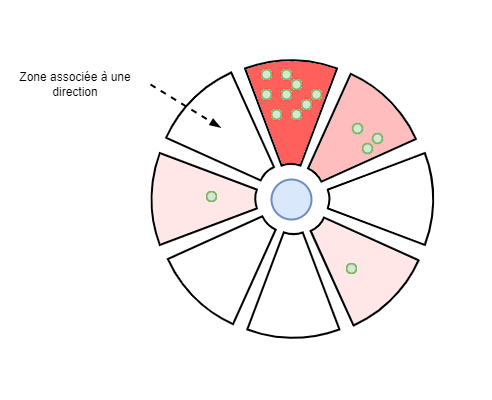
\includegraphics[scale=0.5]{perceptionmap.png}
    \caption{Schéma d'une représentation de la perception map d'une fourmi}
    \label{fig:perception_map}
\end{figure}

\autoref{fig:perception_map} montre ce que "voit" une fourmi qui chercherait la direction vers laquelle elle trouverait le plus de phéromones vertes.
Dans ce schéma, plus une zone est coloriée en rouge, plus elle a de l'importance pour la fourmi.

Dans le calcul de cette perception map, il intervient 3 facteurs différents:
\begin{itemize}
    \item La distance $d$ de la fourmi à la phéromone et la distance de perception $\alpha$ (propriété de la fourmi). \eqref{eq:dist_pheromone}
    \item L'angle $\Delta$ entre le vecteur directeur\footnote{Le vecteur directeur est le vecteur associé à l'angle de la fourmi ou
    autrement dit, la direction dans laquelle elle regarde.} et la direction de la phéromone. \eqref{eq:rot_pheromone}
    \item L'intensité de la phéromone. $e_p$ (avec $p$ la phéromone et $\gamma$ le degré de saturation de l'intensité)
\end{itemize}

\begin{subequations}
\begin{align}
    f(d)=\frac{1}{(1 + e^{\frac{\alpha}{2} - d})} && d,\alpha > 0 \label{eq:dist_pheromone}\\
    r(\Delta)= \frac{1-\left\lvert \Delta\right\rvert}{\pi} && \Delta \label{eq:rot_pheromone}> 0
\end{align}
\end{subequations}

Ces différents facteurs nous permettent de calculer un score $\mu_{p}$ pour chaque phéromone qui représente 
son attractivité pour la fourmi. \eqref{eq:total_pheromone}

\begin{equation}
    \mu_{p} = \sum_{p}{} f(d) \times r(\Delta) \times log_{\gamma}(e_{p})
    \label{eq:total_pheromone}
\end{equation}

Finalement, à chaque direction $u$ nous pouvons récupérer les scores de chaque phéromone $p_{u}$ présente dans cette direction
et les sommer pour obtenir le score total de cette direction qu'on nommera $\lambda_{u}$. \eqref{eq:total_direction}

\begin{equation}
    \lambda_{u} = \sum_{p_{u}}{} \mu_{p_{u}}
    \label{eq:total_direction}
\end{equation}

On peut ainsi attribuer un score d'attractivité qui permettra à la fourmi de savoir quelle direction est la plus intéressante de suivre.
Dans le cas où l'on voudrait que la fourmi soit repoussé par quelque chose, il suffit de faire en sorte que la direction opposée de ce quelque chose
soit intéressante, elle serait donc plus intéressée par la fuite. 

Pour qu'elles évitent les murs, nous avons mis cela en pratique en plaçant trois cercles autour de la fourmi. 
Les cercles qui collisionnent avec un mur vont pousser la fourmi à aller dans la direction opposée.

\begin{figure}[h]
    \centering
    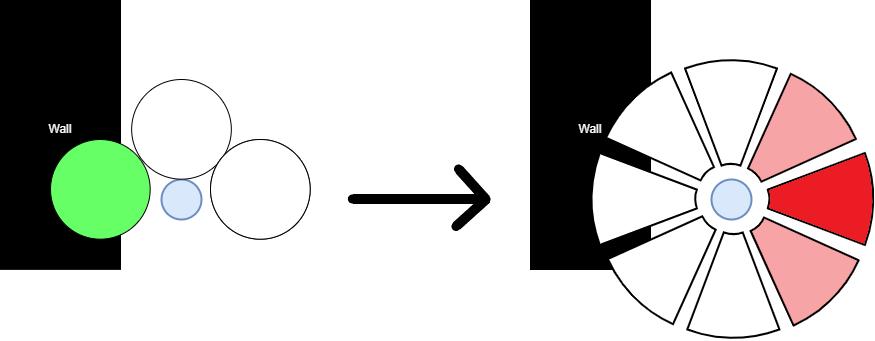
\includegraphics[scale=0.5]{wall_avoidance.png}
    \caption{Schéma d'une représentation de la perception map d'une fourmi lorsqu'elle se rapproche d'un mur.}
    \label{fig:wall_avoidance}
\end{figure}

\subsubsection{Prise de décision de la fourmi}

Maintenant que la fourmi est capable de sentir son environnement proche, il lui faut une manière de modéliser son comportement.
Pour cela, nous avons considérer que la fourmi n'avait que deux phases différentes pour accomplir son objectif:
\begin{enumerate}
    \item La fourmi recherche de la nourriture en suivant éventuellement les phéromones amenant à de la nourriture tout en déposant ceux qui amènent à la colonie.
    \item La fourmi recherche sa colonie en suivant les phéromones la ramenant à sa colonie.
\end{enumerate}

Ces deux phases se répéteront à l'infini de manière successives avec chacune une phase intermédiaire où la fourmi a trouvé ce qu'elle cherchait
et s'y dirige directement. 

\pagebreak

\subsubsection{Machine à états}

Nous avons donc décidé de modéliser cette succession d'états par une machine à états. En effet, cette modélisation nous permet de faire évoluer 
le comportement de la fourmi sans problème. La solution "évidente" à ce problème est le design pattern \textit{State} (États) qui répond
directement à cette problématique et permet de renforcer notre souhait d'avoir un comportement qui peut évoluer facilement.

\begin{figure}[h]
    \centering
    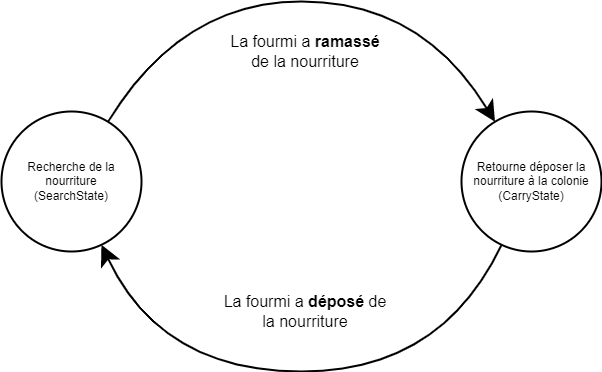
\includegraphics[scale=0.4]{statemachine.png}
    \caption{Schéma de la machine à états}
    \label{fig:state_machine}
\end{figure}

Le design pattern \textit{State} est pratique car à chaque état du comportement, nous pouvons y associer du code à exécuter pour la fourmi via la méthode 
Update vue précédemment mais aussi lorsque la fourmi rentre ou quitte cet état ouvrant ainsi un large panel de possibilités pour les comportements. 

\subsubsection{Entité vivante qui se déplace}

La fourmi ayant pris une décision pour sa direction, il ne reste plus que de s'y déplacer. Cependant, il existe beaucoup de manières de se déplacer
d'un point A à un point B. La fourmi peut par exemple s'y rendre en ligne droite ou alors en ondulant de gauche à droite l'essentiel étant que nous
ne voulons là encore pas nous rendre la vie compliqué plus tard si nous voulons changer cette manière de déplacement.

Nous avons suivi la même philosophie et avons réfléchi à garder une certaine modularité et c'est ici que le design pattern 
\textit{Strategy} (Stratégie) intervient. Il permet de rapidement comparer des méthodes de déplacement en attribuant à chaque colonie 
(ou même à un ensemble de fourmis) une stratégie de déplacement.
Malheureusement, nous n'avons pas eu le temps d'implémenter des stratégies autres que LineStrategy\footnote{Déplacement dans la direction dominante de la PerceptionMap.} 
et WandererStrategy\footnote{Déplacement dans la direction dominante de la PerceptionMap influencée par une variable aléatoire.}.

Pour formuler ça mathématiquement, nous cherchons à chaque tick à calculer la prochaine position $\vec{r_{n+1}}$ de la fourmi à partir
d'une direction dominante $\vec{v}$ qui est donnée par la PerceptionMap calculée précédemment.

La stratégie de déplacement va donc utiliser cette direction $\vec{v}$ pour calculer la vraie direction dans laquelle la fourmi doit aller 
pour respecter la stratégie.

Les fourmis utilisent principalement la stratégie de déplacement WandererStrategy car elle leur permet d'explorer leur environnement tout en prenant
en compte ce qu'elles perçoivent (leur PerceptionMap). Elle utilise deux facteurs en plus: 
\begin{itemize}
    \item $\alpha$ qui représente la part d'aléatoire souhaitée.
    \item $\beta$ qui représente l'influence de l'ancienne direction \footnote{Ce facteur peut aussi être compris comme l'inertie qu'a une fourmi.
    Si on augmente ce facteur, la fourmi aura plus de mal à changer de direction et inversement.}
\end{itemize}

La formule permettant de calculer $\vec{d_{n+1}}$, la direction dans laquelle la fourmi avancera en fonction de ces paramètres est donnée par:

\begin{subequations}
    \begin{align}
        \vec{u}=\alpha \vec{x} + (1 - \alpha) \vec{v} && \text{$\vec{x}$ une direction aléatoire} \\
        \tag{1.4}\vec{d_{n+1}}=\beta \vec{d_{n}} + (1-\beta)u &&  0\leqslant \alpha,\beta \leqslant 1
    \end{align}
\end{subequations}

Ainsi, à chaque tick de la simulation on calcule la nouvelle position $\vec{r_{n+1}}$:

\begin{equation}
    \vec{r_{n+1}} = \vec{r_{n}} + \text{Speed} * \vec{d_{n+1}}
\end{equation}

Après avoir calculé cette nouvelle position, il est tout de même nécessaire de vérifier si la fourmi ne serait pas en collision avec un obstacle en
utilisant son Collider à la nouvelle position. 

\subsubsection{Colonie}

Chaque fourmi est issue d'une seule et unique colonie qui sera l'endroit où elle déposera la nourriture qu'elle trouvera. La colonie tente à chaque tick de
faire apparaître un certain nombre de fourmis en utilisant les ressources qui ont été déposées. C'est une entité très simple dans sa conception car elle
ne sert que "d'usine à fabrication" de fourmis et cela vient aussi du fait que nous ne simulons pas l'intérieur de la colonie.

La colonie a donc a plan de fabrication d'une fourmi ou autrement dit, une liste des ressources nécessaires à la création d'une fourmi et un stock
des ressources qui sont apportés par les fourmis de la colonie.

\subsubsection{Pheromones}

Les phéromones sont le moyen de communication unique des fourmis de notre simulation. Il en existe deux types différentes qui sont diffusées par
les fourmis selon l'état dans lequel elles sont:
\begin{itemize}
    \item Les phéromones de maison
    \item Les phéromones de nourriture
\end{itemize}

Ces deux phéromones permettent donc aux fourmis, selon leur état, de savoir dans quelle direction se trouve leur objectif (colonie ou nourriture).

Il est cependant nécessaire pour les phéromones de ne pas être infinies car les fourmis pourraient s'intéresser à des phéromones inutiles car trop anciennes, 
nous obligeant donc à implémenter un système de minuteur qui à sa fin déclencherait la suppression de la phéromone.

Nous avons donc fait en sorte que lorsqu'une fourmi émet une phéromone, elle lui donne son intensité et cette intensité sera la valeur qui servira de décompte
pour la phéromone. En effet, nous décrémentons l'intensité à chaque tick jusqu'à atteindre 0 et lorsque l'intensité est nulle il est effectivement normal 
de supprimer la phéromone de la simulation car elle n'a plus aucun impact sur celle-ci.

Il a cependant fallu faire attention à la durée entre les deux types de phéromones car nous avons remarqué que celles amenant à la nourriture n'avaient 
pas autant d'intérêt à rester longtemps comparées à celles menant à la colonie car contrairement à celle-ci, la nourriture est plus susceptible de 
disparaître et il est donc contre-productif de garder des phéromones amenant à une source de nourriture épuisée.

Pour améliorer les performances de la simulation, nous avons implémenté un système de fusion de phéromones lorsqu'elles sont trop proches car malgré 
le fait qu'ils comptaient pour deux entités différentes, la fourmi ne pouvait pas faire la distinction entre deux phéromones à seulement quelques 
nanomètres d'écart.

\subsubsection{Ressources}

Les ressources sont l'objectif des fourmis en état de recherche. Nous avons cependant une distinction entre les objets \textbf{Ressource} et 
\textbf{Entité de ressource}. Pour donner un exemple, imaginons une ressource de pomme dans le monde de la simulation. Ici, la \textbf{Ressource}
serait l'idée d'une ressource pomme tandis que l'\textbf{Entité de ressource} serait la pomme réellement posée dans la simulation, récupérable par 
les fourmis.

Cette distinction nous permet d'avoir plusieurs dépôts de ressources représentant la même ressource. Mis à part cela ces objets sont très simples
et n'ont aucune comportement propre.

\section{Application}

Maintenant que nous avons présenté la partie moteur de simulation de notre application, nous allons expliquer l'architecture de la partie applicative du projet.
Pour rappel, le projet était principalement centré sur le moteur de simulation mais la partie applicative était importante car c'est elle qui permet à l'utilisateur 
d'interagir simplement avec le moteur. 

\subsection{Présentation de la structure}

L'application utilise donc le framework MonoGame (anciennement XNA) et bien que ce framework est très simple d'utilisation, cela ne nous a 
pas empêché de devoir concevoir une structure robuste pour permettre d'afficher de multiples objets différents à l'écran.
Nous avons grossièrement deux catégories d'éléments à afficher à l'écran:
\begin{itemize}
    \item Les entités de la simulation
    \item Les éléments de l'interface
\end{itemize}

Ces deux types d'objets sont certes différents mais il est possible de trouver propriétés communes aux objets de rendu de chacun.

Nous avons pour cela créer un adaptateur des objets de la simulation pour qu'ils soient compatibles avec nos méthodes de rendu 
utilisant MonoGame. Ainsi, les entités sont munis d'un analogue Renderer dans la partie application qui est chargé d'afficher la dite 
entité à l'écran.

Par souci de simplicité, nous avons fait en sorte que chaque composant serait lui même responsable de s'afficher sur l'écran en utilisant les
objets de rendu qu'il a à disposition (SpriteBatch\footnote{Element donné par MonoGame pour dessiner des Sprites (des images) à l'écran. 
\url{https://docs.monogame.net/api/Microsoft.Xna.Framework.Graphics.SpriteBatch.html}} et GraphicsDeviceManager\footnote{API graphique plus
bas niveau que SpriteBatch mis à disposition par MonoGame. Permet de dessiner directement sous la forme de vertex, plus proche d'une manière "à la 
OpenGL". \url{https://docs.monogame.net/api/Microsoft.Xna.Framework.GraphicsDeviceManager.html}"}).

Chaque Renderer utilisera donc ces objets avec des informations lui indiquant la position sur l'écran à laquelle il doit s'afficher pour
lui même se rendre. D'autres applications font la méthode inverse où un objet de rendu principal utilise les informations qui lui sont 
données pour afficher tous les objets.

\begin{figure}[h]
    \centering
    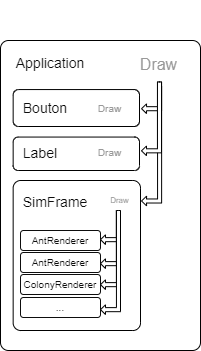
\includegraphics[scale=0.8]{application_draw.png}
    \caption{Schéma de la chaîne de rendu}
    \label{fig:draw_chain}
\end{figure}

\autoref{fig:draw_chain} montre comment la méthode \textit{Draw} de MonoGame est distribuée parmi tous les objets à afficher pour qu'eux-
mêmes s'affichent.
Il y a cependant un élément en particulier qui est très important qui n'est autre que l'espace de rendu de la simulation nommée \textbf{SimFrame}.
Cet élément est particulier car sa méthode Draw ne fait que transmettre la cascade d'appel à la méthode de rendu aux Renderers des entités
de la simulation.

Ainsi, avec chaque renderer qui est associé à une entité à afficher de la simulation, nous avons une représentation lisible de ce qu'il
se passe dans la simulation. Le fait qu'il existe un renderer pour une entité nous permet si nous le souhaitons de faire un rendu différent
sur des entités possédant une classe de rendu similaire (des couleurs différentes pour des fourmis).

\subsubsection{Elements d'interface}

Pour ce qui est de l'interface utilisateur, nous avons implémenté quelques classes d'éléments pour l'application.

\paragraph{Label}
Cet élément permet d'afficher du texte là où nous voulons sur l'écran pour donner à l'utilisateur des informations supplémentaires.

\paragraph{Bouton}

Nous avons évidemment implémenté un système de boutons qui nous permet de rajouter la possibilité à l'utilisateur de déclencher des actions à l'aide d'un 
simple clic. Nous avons là encore fait en sorte de nous ouvrir le plus de possibilités pour des extensions futures et avons donc mis le plus d'évènements 
possibles qui sont:
\begin{itemize}
    \item Début de clic sur le bouton
    \item Bouton cliqué (maintenu)
    \item Clic relevé
\end{itemize}

\begin{figure}[h]
    \centering
    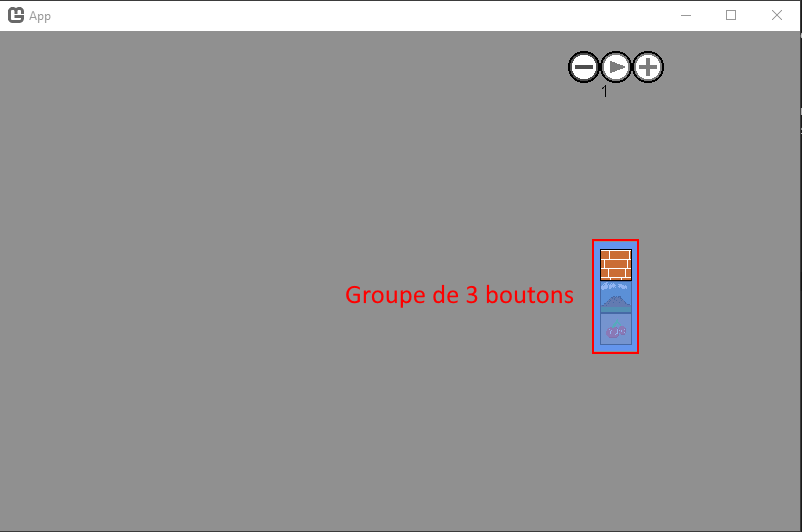
\includegraphics[scale=0.5]{button.png}
    \caption{Exemple des boutons dans l'application}
    \label{fig:button_example}
\end{figure}

\pagebreak

\paragraph{Sélecteur de vitesse}

Le sélecteur de vitesse permet à l'utilisateur de choisir la vitesse de simulation cible à laquelle le moteur doit
aller. Il est composé de trois boutons:
\begin{itemize}
    \item Ralentir
    \item Accélérer
    \item Mettre en pause / Reprendre
\end{itemize}

\begin{figure}[h]
    \centering
    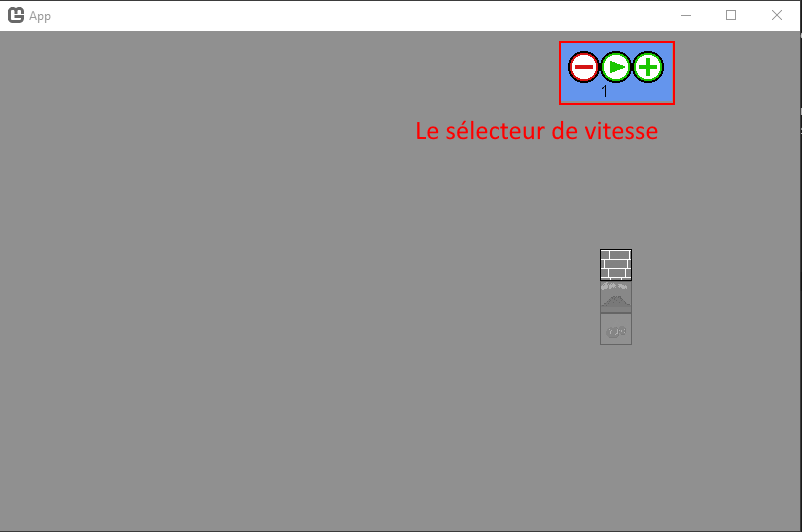
\includegraphics[scale=0.3]{speedslider.png}
    \caption{Sélecteur de vitesse dans l'application}
    \label{fig:speedslider_example}
\end{figure}


\paragraph{SimFrame}

La fenêtre de simulation et les éléments qui la composent (les EntityRenderer) doivent répondre à une problématique supplémentaire.
Le monde de la simulation étant dans un système de coordonnées totalement indépendant des pixels dans lequel les éléments graphiques sont
rendus, il faut faire une adaptation de ces coordonnées pour qu'à partir de coordonnées dans le monde, nous sachions où afficher l'objet sur l'écran.

\begin{figure}[h]
    \centering
    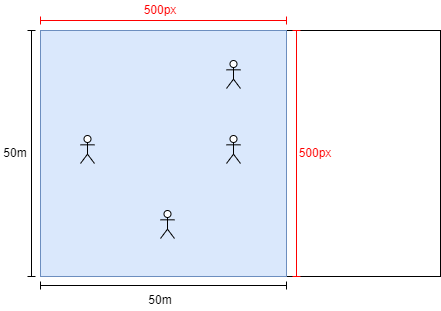
\includegraphics[scale=0.7]{simframe.png}
    \caption{Représentation des différents systèmes de coordonnées concurrents dans l'application}
    \label{fig:simframe}
\end{figure}

Il est aussi nécessaire de garder le ratio d'affichage initial du monde pour éviter les déformations. Cela veut dire qu'un monde carré 
doit être affiché sous la forme d'un carré et ne peut donc pas juste simplement remplir toute la fenêtre. Nous avons aussi fait le choix 
d'inverser l'axe vertical de rendu car, comme dans beaucoup de frameworks de rendu graphique, l'axe vertical est du haut vers le bas et non du 
haut vers le bas.

\chapter{Réalisation}

\paragraph{}
Ce chapitre présente le déroulement du projet, les aléas qui sont apparus au cours du 
développement et d'autres aspects de développement qu'il nous a semblé 
utile de faire apparaître.

\section{Choix des outils et technologies}

\subsection{Outils de collaboration}

Lors des projets de 3\textsuperscript{ème} année, nous avons beaucoup appris sur comment utiliser
Git. Nous avons choisi d'utiliser \textbf{GitHub} en tant qu'outil de versionnage en raison de notre aise avec et
car le site possède un grand nombre de fonctionnalités nous permettant de mieux communiquer entre
nous.

Lors du projet nous avons adopté une méthode de travail basé sur le \textbf{GitFlow}\footnote{Une méthode de travail où on sépare chaque feature ou fix dans une branche séparée.
Ensuite une fois la feature finie, on créé un \textit{Merge Request} afin de demander la validation des autres développeurs.} avec pour seule nuance que nous n'avions pas de branches \textit{dev} ou \textit{release}
mais plutôt toute modification se fusionnait directement à la branche \textit{main}.

Cela avait pour avantage de nous permettre de suivre les avancements de l'autre personne et de pouvoir 
apporter des suggestions ou des commentaires sur ce qui avait été fait. 
En fin de compte l'utilisation de ce workflow nous a permis de connaître et comprendre 
les parties de codes que l'autre écrivait et donc de pouvoir beaucoup avancer chacun de notre
côté en ne laissant pas l'autre personne à l'abandon.

\begin{figure}[h!]
\centering
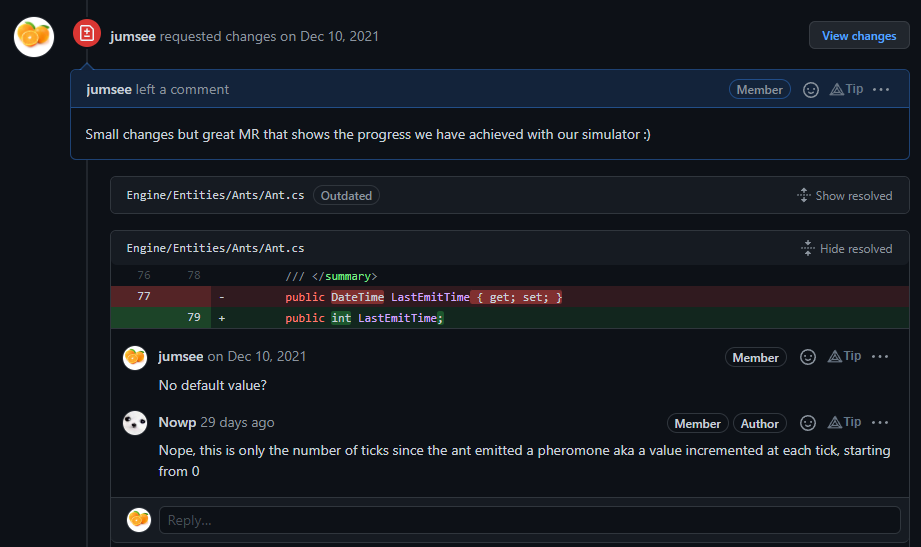
\includegraphics[scale=.5]{merge_request.png}
\caption{Exemple de commentaire sur une merge request pour l'ajout de la disparition des phéromones.}
\label{fig:MergeRequest}
\end{figure}

En plus des merge requests, GitHub nous permet de créer des \textit{issues}\footnote{Ici fait référence 
au mot anglais issue qui signifie un problème à résoudre.}.
Ces \textit{issues} peuvent être considérées comme des tâches qu'il reste à faire. Au sein de GitHub, nous
pouvons à tout moment nous approprier une tâche afin d'indiquer qu'on a commencé à travailler dessus. Cela 
permet de bien savoir ce sur quoi l'autre personne travaille et également d'avoir un aperçu rapide de ce qu'il reste à faire dans le projet.

Il est évident que le nombre d'issues que nous avions au début du projet n'est pas le même qu'à la fin. Au cours du projet nous
pouvions découvrir des aspects du code à réparer (dans ce cas l'issue serait plutôt un \textit{bug report}) ou encore des fonctionnalités
importantes auxquelles nous n'avions pas pensé.

Les issues nous ont également permis de débattre entre nous sur quelle serait la meilleure solution à un problème. Essentiellement, toute utilisation
de GitHub est dans l'objectif de faciliter la communication et le fait que tout soit bien répertorié nous assure de ne pas oublier des échanges que 
nous aurions pu avoir.

Ces issues apparaissent au sein de Kanbans \footnote{Au sein de ce projet le Kanban était notre tableau de bord et nous permettait de suivre 
l'avancement et de savoir ce qu'il restait à faire. Plus d'informations : \url{https://en.wikipedia.org/wiki/Kanban_(development)}.}
qu'on retrouve directement intégré à GitHub. Nous avions deux Kanbans, un pour l'application et l'autre pour le moteur de simulation comme ces deux éléments peuvent avancer très facilement en parallèle.

Dans \autoref{fig:Kanban} on peut voir les tâches qui sont en cours de développement et ceux qui sont prêts à être review.

\begin{figure}[h]
\centering
\includegraphics[scale=.3]{kanban.png}
\caption{Exemple du tableau de bord côté Application}
\label{fig:Kanban}
\end{figure}

Un autre élément que nous avons utilisé avec GitHub est la fonctionnalité d'intégration continue. En effet, nous avons configuré notre projet 
pour lancer tous les tests unitaires à chaque commit effectué sur une branche.
Cela nous permettait de tout de suite nous rendre compte qu'une régression sur le programme était apparue et nous évitait d'accumuler des erreurs.
Ainsi, pour fusionner les changements il était nécessaire que d'une part nous ayons la totalité des tests unitaires qui réussissent et en plus de cela,
d'avoir l'approbation de l'autre personne pour pouvoir procéder à la fusion dans le main.

\subsection{Langages et Langues}

Le choix du langage de programmation à utiliser était une décision importante à prendre. Nous avons décidé de faire ce projet en C\# car c'est un langage que nous
n'avons pas encore pu utiliser au sein du parcours à Polytech. Nous étions au courant du fait que le C\# était très proche du Java et donc il n'y avait pas
d'inquiétudes sur notre capacité à l'apprendre rapidement. Le C\# reprend aussi les concepts de machine virtuelle qui existent en Java ce qui permettrait de build et lancer le projet
sur n'importe quel système d'exploitation grâce à .NET.
De plus, le C\# est un langage que nous avions pu utiliser lors de petit projets sur Unity mais jamais sur un gros projet comme celui-ci. 
A l'intérieur de C\# le standard de documentation utilisé est XMLdoc\footnote{Plus d'informations : 
\url{https://docs.microsoft.com/en-us/dotnet/csharp/language-reference/xmldoc/}.}.

Ensuite, il a fallu que nous nous décidions quelle convention de nommage nous allions utiliser. 
Malgré notre envie d'utiliser celle présentée par notre enseignant en cours de C++ en 3\textsuperscript{ème} année, nous avons découvert la convention 
proposée par Microsoft pour le C\#\footnote{Plus d'informations : \url{https://docs.microsoft.com/en-us/dotnet/csharp/fundamentals/coding-style/coding-conventions}} qui nous a particulièrement plu.
Dans une volonté de vouloir rester polyvalent et malléable en terme de méthodes de travail, nous avons décidé d'adopter cette convention.

Pour ce qui est de la langue dans laquelle nous avons codé, nous avons décidé de tout faire en Anglais pour que le code soit facilement
transmissible et exploitable par d'autres personnes dans le monde, chose qui dans le contexte de la mondialisation reste très important.

\subsection{Librairie de tests unitaires}

Il existe plusieurs librairies de test au sein de l'environnement .NET. Les plus utilisés sont XUnit, NUnit et MSTest.
La bibliothèque que nous avons choisi d'utiliser est XUnit en raison du fait que l'un d'entre nous l'avait déjà utilisé au sein d'un projet personnel.

\subsection{Framework d'affichage}

Au lancement du projet, nous avons dû réfléchir à quel framework utiliser pour faire l'affichage de la simulation.
Dans un premier temps, nous nous étions intéressé à Avalonia, un framework cross-platform qui est un successeur spirituel de WPF\footnote{WPF ou Windows Presentation Foundation est un framework 
utilisé pour la création d'interfaces graphique. Aujourd'hui ce framework a beaucoup vieilli et est en train d'être remplacé par des frameworks plus modernes tels que Avalonia.}.
On s'est rendu compte qu'Avalonia n'était pas du tout ce qu'on recherchait comme il ne servait qu'à faire des interfaces graphiques type Swing et 
était très peu utilisable pour l'affichage en temps réel (jeu vidéo ou simulation).

Nous avons donc dû rechercher une solution alternative et c'est là que nous avons découvert MonoGame. 
MonoGame est un framework graphique open-source utilisé principalement pour des jeux comme son nom l'indique et qui est basé
sur XNA (un framework développé par Microsoft et abandonné depuis 2013). 
Après avoir consulté la documentation et avoir fait des recherches dessus, MonoGame est le framework que nous avons décidé d'utiliser. 
En complément de MonoGame, l'ensemble des textures présents dans le projet ont été créé à la main avec Piskel\footnote{Outil gratuit de dessin de PixelArt en-ligne. 
Plus d'informations : \url{https://www.piskelapp.com/}.}. 

\section{Moteur}

\subsection{Abstraction des Colliders}

Lorsque nous avons codé les colliders, nous nous sommes rendu compte que la manière initiale dont nous l'avions conçu
faisait qu'il y avait énormément de duplication de code ce qui le rendait difficilement maintenable.

Exemple : Pour tester la collision entre un cercle et un rectangle il y a deux cas. 
\begin{itemize}
    \item Premier cas : le cercle appelle sa méthode CheckCollision en passant le rectangle en paramètre.
    \item Second cas : le rectangle appelle sa méthode CheckCollision en passant cette fois-ci le cercle en paramètre.
\end{itemize}

La solution à cela était de déplacer les méthodes de collision dans une méthode statique et qu'ensuite chaque collider fasse appel à la méthode
qu'il a besoin.

\subsection{Transforms et Colliders}

Comme indiqué précédemment, l'objet Transform que nous avons utilisé est inspiré de celui qu'on retrouve sur Unity. Un autre concept que nous avons voulu reprendre d'Unity est le fait qu'un
collider puisse posséder son propre transform ce qui lui permet d'avoir une position autre que celle de l'entité à laquelle il est attaché. Ca permet aussi aux colliders d'exister sans être forcément
lié à une entité.

Au début du projet, nous avions pour intention d'implémenter cela dans le moteur de simulation. 
Un collider aurait donc un transform et s'il est rattaché à une entité, le transform du collider serait en coordonnées relatives (pour obtenir sa position réelle, il faudrait faire Entity.Transform + Collider.Transform).
Il s'avère que cette solution ajoute beaucoup de complexité aux calculs de collision et ne serait même pas utile au sein de la simulation. Nous avons donc pris la décision d'enlever cette 
fonctionnalité et de lier fortement les colliders aux entités en leur faisant prendre le transform de l'entité à laquelle ils sont rattachés.

\subsection{Temps de simulation ou temps réel ?}

Une erreur gigantesque que nous avons commise est le fait que nous avons ajouté des éléments qui dépendaient du temps réel dans le moteur de simulation (un exemple serait le temps de disparition des phéromones).
Le problème ici vient du fait que nous voulions permettre aux utilisateurs de ralentir, accélérer ou mettre en pause la simulation.

\begin{figure}[h]
    \centering
    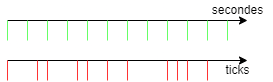
\includegraphics[scale=1]{ticks_secondes.png}
    \caption{Exemple d'appels de la méthode Update en temps réel et en temps de simulation.}
    \label{fig:ticks_secondes}
\end{figure}

Les lignes rouges dans \ref{fig:ticks_secondes} représentent des appels à Update. On voit que la méthode n'est pas appelé de manière uniforme ce qui cause des décalages si on tente de changer la vitesse de la simulation.

Malheureusement, mettre en pause la simulation ne met pas en pause la vrai vie ! Il y a donc une désynchronisation qui se déroule et qui peut causer des problèmes de cohérence et d'intégrité.
La solution à ce problème est évidente, il faut décompter tout en nombre de \textit{ticks}, c'est à dire, de fois où la méthode Update du World est appelée. 
Cela fait que chaque phéromone possède un compteur pour sa disparition qui décroît d'une unité à chaque tick. Cela permet de garder la cohérence dans le cas de modification de la vitesse de la simulation.

\subsection{Optimisation}

La problématique de l'optimisation de la simulation a été un enjeu très important pour nous tout au long du projet. Nous avons dû réfléchir sur les implémentations qui ont été faites afin de vérifier qu'elles ne 
faisaient pas chuter les performances. Que ce soit au niveau de quel type d'objet nous utilisions du C\# ou encore vérifier qu'on ne remplissait pas inutilement le garbage collector 
\footnote{Le garbage collector est un gestionnaire de mémoire qui supprime et désalloue automatiquement des objets quand ils ne sont plus référencés par le programme. 
Plus d'informations sur comment il fonctionne en .NET : \url{https://docs.microsoft.com/en-us/dotnet/standard/garbage-collection/fundamentals}}.
Quand on parle de simuler une quantité de fourmis qui peut aller dans les milliers, sachant que chaque fourmi doit évaluer son environnement et prendre des décisions, les performances chute très rapidement.

Nous présenterons dans cette partie les principales optimisations que nous avons effectués pour augmenter au maximum le nombre de fourmis que le simulateur peut supporter.

\subsubsection{Structures de données}
Un autre élément important dans l'optimisation de la simulation a été le choix des structures de données. 
On s'est rendu compte que l'objet List<T> en C\# est très efficace lorsqu'on traite des liste de peu d'éléments
mais, quand il y a un grand nombre d'éléments dans la liste, l'objet HashSet (objet dictionnaire) est beaucoup plus rapide à utiliser
\footnote{Nous avons basé cette observation sur le poste suivant : \url{https://stackoverflow.com/a/10762995/15541425}} mais prend plus de mémoire.
Dans notre cas la performance est critique donc nous avons introduit le HashSet là où il y avait des listes de grande taille, 
c'est à dire principalement dans la récupération d'éléments pour former le perception map d'une fourmi.

On pourrait donc se demander pourquoi nous n'avons pas utilisé un HashSet pour le découpage du monde en régions ? 
La réponse est simple, pour les objets qui seront accédé souvent le type primitif jagged array
\footnote{Plus d'informations : \url{https://docs.microsoft.com/en-us/dotnet/csharp/programming-guide/arrays/jagged-arrays}}
en C\# est ce qui est conseillé en raison de sa performance.

Enfin, la dernière optimisation que nous avons fait pour les structures de données est au niveau des Properties.
Un Property\footnote{Plus d'informations : \url{https://docs.microsoft.com/en-us/dotnet/csharp/programming-guide/classes-and-structs/properties}}
en C\# est un type de déclaration de variable qui permet de générer automatiquement les accesseurs d'une classe.
Ce type permet de simplifier le code et d'éviter aux développeurs d'écrire des méthodes qui vont juste allonger le code pour pas grand-chose.

Nous avons aussi remarqué que les properties\footnote{Documentation C\# sur les Properties : \url{https://docs.microsoft.com/fr-fr/dotnet/csharp/programming-guide/classes-and-structs/properties}}, malgré leur intérêt évident, sont beaucoup plus lentes que des attributs standards
du fait qu'elles ne sont que des manières de générer les getter et setter. 
Il a donc été très avantageux pour nous de ne pas utiliser de Property pour les éléments qui sont utilisés fréquemment.


\subsubsection{Découpage par régions}

Le découpage par régions est l'optimisation la plus "simple" mais évidente que nous avons ajouté.

\begin{figure}[h]
    \centering
    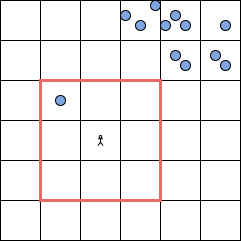
\includegraphics[scale=1]{decoupage_region.png}
    \caption{Exemple de cas où l'optimisation par découpage en régions est très utile.}
    \label{fig:decoupage_region}
\end{figure}

Dans la figure \ref{fig:decoupage_region} on observe que la plupart des entités sont loin de l'individu au centre, l'optimisation par régions permet de ne pas les prendre en compte et donc de ne faire des calculs
de collision qu'avec les objets dans la zone de perception de l'individu.
Nous avons implémenté ce découpage en permettant aux fourmis de récupérer les entités qui sont dans une certaine zone autour d'eux (en nombre de régions ou en distance réel dans le monde).
Cette optimisation nous a apporté un énorme gain en performances et a notamment rendu la présence d'un grand nombre de fourmis et de phéromones peu impactant sur les performances.


\pagebreak

\subsubsection{Fusion de phéromones}
Un autre problème que nous avons remarqué au même moment que nous avons fait le découpage des régions est le fait qu'après avoir laissé la simulation ouverte pendant longtemps, les fourmis
auront émis un grand nombre de phéromones. Cela ralentissait énormément la simulation en raison du nombre d'entités qui existaient dans le monde. Il fallait donc trouver une solution permettant
d'avoir beaucoup de phéromones sans pour autant condamner la simulation à perdre en performances après un certain temps.
Notre solution ici était de faire une fusion de phéromones si elles sont assez proches. La fusion de deux phéromones combine leur attirance pour les fourmis et donc permet de garder les informations
tout en optimisant plus la simulation. Cette fusion avait une limite supérieure ce qui empêche d'avoir des phéromones qui persistent extrêmement longtemps.
Cette optimisation, combinée avec le découpage en régions, nous a apporté la plus grande augmentation en vitesse de simulation.

\subsubsection{Garbage Collector}
Nous avons également dû travailler sur l'optimisation du garbage collector. Si trop d'objets sont créés et supprimés, le garbage collector va devoir travailler plus souvent pour les allouer et les désallouer
ce qui influe beaucoup sur les performances.  

\begin{figure}[h]
    \centering
    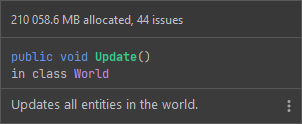
\includegraphics[scale=1]{garbage_collector.png}
    \caption{Mémoire allouée par la méthode main après 10 minutes de simulation (avant les optimisations).}
    \label{fig:garbage_collector}
\end{figure}

On voit sur la figure \ref{fig:garbage_collector} qu'après très peu de temps, la mémoire qu'aura alloué le simulateur est très élevée.
Afin de résoudre ce problème, nous avons utilisé les outils de profiling de mémoire qu'on retrouve dans notre IDE
\footnote{Pour ce projet, nous avons utilisé Rider qui est un IDE pour le C\# développé par JetBrains.}.

L'optimisation ici est simple, il nous a suffit de prioriser la réutilisation de variables et éviter de les déclarer et détruire trop souvent.
Un exemple pertinent de cela est pour l'objet PerceptionMap qui avant, était recréé à chaque mise à jour du monde. Après l'optimisation, la perception map est stockée dans la fourmi
et est simplement remise à zéro à chaque mise à jour du monde. 

Suite à ces optimisations, l'outil de vérification de mémoire dans Rider ne nous affichait plus d'avertissements et donc nous pensons avoir totalement résolu le problème.

\section{Application}

\subsection{Renderers}
Une autre hésitation que nous avons eue durant le projet était au niveau de comment gérer la structure de rendu dans l'application et comment 
faire l'association entre une entité du moteur et ce qu'on dessine à l'écran. Au début, nous avions pensé à créer une classe qui s'occuperait de faire le rendu des
entités en parcourant la liste présente dans l'objet World (voir la figure \ref{fig:renderer_logic_1}). 

\begin{figure}[h]
    \centering
    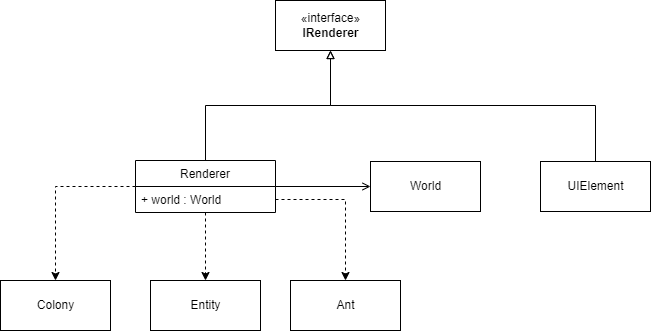
\includegraphics[scale=0.5]{renderer_logic_1.png}
    \caption{La structure initiale que nous avions prévu d'utiliser (one-to-all). }
    \label{fig:renderer_logic_1}
\end{figure}

Avec l'architecture montrée dans \autoref{fig:renderer_logic_1}, on voit que l'objet Renderer serait rapidement devenu peu pratique 
à utiliser et à modifier.

En fin de compte, nous avons trouvé que cette solution était peu pratique car si nous voulions un comportement 
de rendu différent pour des objets d'une classe particulière, il aurait fallu faire une disjonction de cas par rapport au type. Cela nous aurait fait finir avec
une méthode très longue qui aurait été un véritable cauchemar à gérer. 

Nous avons donc pris la décision logique de plutôt créer des renderers génériques pour les entités n'ayant pas besoin de comportement 
en plus et dans le cas d'entités comme les fourmis ou la colonie qui avaient des textures ou comportements différents, nous pouvions créer un renderer
précis juste pour eux (voir la figure \ref{fig:renderer_logic_2}).

\begin{figure}[H]
    \centering
    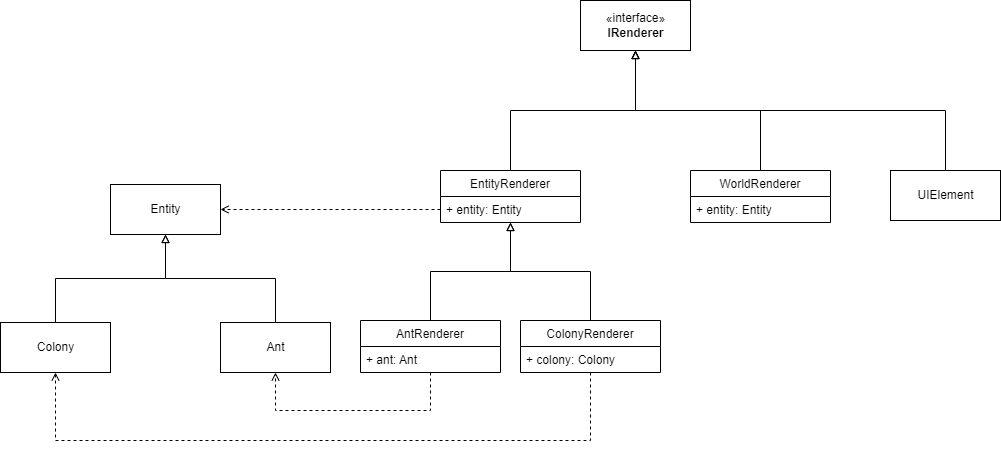
\includegraphics[scale=0.3]{renderer_logic_2.png}
    \caption{La structure finale que nous avons utilisé (one-to-one). Elle permet facilement d'aller modifier ce qu'on a besoin pour l'affichage d'un type d'objet précis.}
    \label{fig:renderer_logic_2}
\end{figure}

\subsection{Fichier de propriétés}
Afin de faciliter la configuration de la simulation, nous avons utilisé un fichier properties
\footnote{Nous avons utilisé une implémentation de gestion de fichier properties postée sur StackOverflow car en Java il existe une implémentation native qu'on ne retrouve pas en C\# : 
\url{https://stackoverflow.com/questions/485659/can-net-load-and-parse-a-properties-file-equivalent-to-java-properties-class\#answer-7696370}}
qui permet de spécifier les changements qu'on veut ajouter comme par exemple la vitesse des fourmis
ou les ressources nécessaires pour qu'une colonie fasse apparaître une fourmi. A l'origine, nous avions prévu de permettre la configuration de ces options directement dans la simulation, mais,
le fait d'utiliser MonoGame nous a imposé de créer les objets de saisie de texte à la main. Nous avons décidé que cela serait une trop grosse perte de temps et ne rentrait pas dans 
le cadre du projet. Le fichier Properties a été donc un gain de temps énorme pour nous, comparé à l'alternative.

\subsection{Pipeline de contenu}
Un des avantages de MonoGame était le principe d'importation de textures (ou content pipeline) qui était très pratique à utiliser. Pour importer une texture dans la simulation nous devions ouvrir l'éditeur 
MGCB\footnote{MonoGame Content Builder(MGCB) est un utilitaire qui permet de simplifier l'importation de textures dans le framework MonoGame. Plus d'informations : \url{https://docs.monogame.net/articles/tools/mgcb_editor.html}}
.Cet éditeur nous permettait de simplement spécifier un fichier .png et une fois que nous avions build le projet, le texture serait ajouté au projet et pouvait être exploité en l'important en une ligne : 
\begin{verbatim}
    Texture2D maTexture = Content.Load<Texture2D>("chemin/vers/texture");
\end{verbatim}

\section{Tests}

Malgré notre envie d'écrire des tests, nous nous sommes rendu compte que dans notre projet, il était facile de tester les classes simples comme les colliders ou les transforms
mais, dès qu'on voulait tester des choses plus avancées comme le comportement des fourmis, il était difficile d'écrire des tests qui n'étaient pas juste une perte de temps ou redondants.
C'est pourquoi nous n'avons pas pu écrire autant de tests que ce qu'on visait au départ. De plus, la partie application du projet ne contient aucun test, nous avons testé à la main les interfaces comme il n'y
avait pas beaucoup de possibilités à tester.

En revanche, les choses que nous avons testées nous ont permis de détecter des problèmes qui auraient été compliqués à trouver sinon (comme par exemple des problèmes avec nos formules de collision)
\footnote{La liste des tests qui ont été faits peut être trouvée en annexe.}.

\chapter{Résultats et perspectives}

\section{État des lieux}

Après 6 mois de travail, nous avons abouti sur un logiciel qui peut simuler des colonies de fourmis et leurs interactions avec leur environnement.
Notre simulateur nous permet de placer des murs, des colonies et de la nourriture. 
Les fourmis ont le comportement que nous avions prévu, c'est à dire, elles cherchent la nourriture et une fois trouvée, elles ramènent à la colonie et elles avertissent les 
autres fourmis de ce qu'elle a trouvé par le biais des phéromones.
L'application accompli également son rôle d'interface entre le simulateur et l'utilisateur. On peut ensuite régler la vitesse de la simulation qui sera limitée par la vitesse de l'ordinateur quand on l'augmente.
Nous pensons avoir écrit du code qui permet d'ajouter de fonctionnalités en plus à la simulation sans poser de problèmes.

En tout, nous pensons avoir bien réussi à accomplir les objectifs initiaux du projet.

\section{Apports}

Grâce à ce projet, nous avons appris et renforcé beaucoup de connaissances différentes que nous avions vu à Polytech mais aussi 
dans nos projets personnels. 

Tout d'abord, nous avons beaucoup progressé dans la maîtrise des de conduite de projet. La mise en place d'un répertoire
GitHub et son utilisation tout au long du projet pour discuter, nous assigner des tâches et connaître l'avancement global du projet a été un élément essentiel
et tout aussi important que la programmation elle-même. Ensuite, nous avons pu aussi nous entraîner à une étape très importante d'un 
projet qui est la configuration des librairies et de l'environnement de travail.

Pour ce qui est des compétences plus techniques, nous avons pu approfondir nos connaissance en C\# et surtout mettre en application
l'utilisation des design patterns vus en cours de qualité logicielle. Nous avons été amené à nous poser des questions d'optimisation
et sur la complexité de nos algorithmes. Cela nous a aussi poussé à utiliser des outils de profiling accompagnés aux outils de debugging dont nous
avions tout de même l'habitude.

Étonnamment, nous avons aussi appris l'utilisation de LateX pour réaliser ce rapport et découvert les miracles que cette technologie est capable 
de réaliser alors que nous ne pensions pas l'utiliser.

Enfin, nous avons bien évidemment pu en apprendre bien plus sur ces créatures pleines de surprises que sont les fourmis et cela nous a motivé 
à nous renseigner d'avantage sur le domaine du biomimétisme en général.


\section{Évolutions possibles}

Bien que nous soyons fiers de notre simulation, il y a une multitude d'améliorations et d'évolutions qui sont possibles.

\subsection{Comportement des fourmis}

Une amélioration conséquente que nous pourrions faire serait de réparer les problèmes qui existent avec le comportement des fourmis.

\subsubsection{Bouclage}

Un problème avec le comportement actuel est le fait que certaines fourmis vont faire du Bouclage. Pour plus détailler, il s'agit du cas
où une fourmi a trouvé de la nourriture et elle commence à suivre une fourmi qui cherche de la nourriture ou tout simplement un circuit de phéromones. 
Les fourmis ont un risque de commencer une boucle où elles vont chacune se suivre et ne jamais pouvoir en sortir.
Bien que ce phénomène existe dans la vrai vie\footnote{Voir : \url{https://youtu.be/LEKwQxO4EZU}}, ce n'est pas censé arriver aussi fréquemment que dans notre simulation.
Une solution serait de faire en sorte que la fourmi puisse abandonner sa recherche ce qui sortirait les fourmis du cycle.

\subsubsection{Les Murs}
Un autre problème est le fait que les fourmis voient les phéromones à travers des murs. Il peut arriver qu'elles se ciblent sur un morceau de 
nourriture en particulier de l'autre côté d'un mur et soient donc bloquées contre le mur.
Il faudrait donc vérifier la présence d'un mur avant de passer en TargetState et permettre à la fourmi d'avancer sur la nourriture qu'elle voit.

\subsubsection{Phéromones}
Enfin, la dernière amélioration en lien avec le comportement des fourmis est le fait que parfois les fourmis ont du mal à remonter la trace des phéromones qui les mènerait à la bonne destination et elles finissent par
se perdre sur le chemin du retour à leur colonie. Il peut aussi arriver qu'une fourmi suive des phéromones dans la mauvaise direction et donc les conduire à leur colonie et non pas à la nourriture (ou inversement).

\subsection{Properties}
Comme énoncé précédemment, il serait possible de rajouter un endroit à l'intérieur de la simulation qui permet de modifier les règles de la simulation.
On pourrait aussi rajouter de la personnalisation en plus dans l'application (liste non-exhaustive) : 
\begin{itemize}
    \item Déterminer quelle quantité de nourriture est dans l'entité de nourriture qu'on pose.
    \item Pouvoir placer des colonies qui ont des propriétés différentes.
    \item Pouvoir modifier la couleur des fourmis d'une colonie.
    \item Une brosse pour poser des éléments plus gros (une plus grosse colonie ou un plus gros mur par exemple).
    \item La possibilité de pouvoir zoomer dans la simulation pour que la taille de monde maximum ne dépende pas de la taille de son écran.
\end{itemize}

\subsection{Optimisation}
Une autre fonctionnalité intéressante dont nous sommes déçus de ne pas avoir pu ajouter est le multithreading. En effet l'ajout du multithreading (CPU ou GPU) dans les calculs permettrait d'afficher 
encore plus d'entités dans la simulation. On pourrait envisager une distribution du travail par régions 
(chose qui se rapprocherait du calcul d'une fractale de Mandelbrot\footnote{Plus d'informations : \url{https://fr.wikipedia.org/wiki/Ensemble_de_Mandelbrot}} par exemple).
Il faudrait donc rajouter des protections contre les problèmes de concurrence et rendre le logiciel thread-safe. 

Enfin, malgré le fait que nous sommes contents d'avoir pu apprendre le C\#, il est fort probable que si nous avions fait le projet en C++ 
ou dans un autre langage qui est plus proche de la machine, l'application aurait été plus rapide et moins complexe à optimiser.


\subsection{Fonctionnalités liés au monde}
Ensuite, une autre addition qui pourrait être intéressante est le fait de pouvoir importer et exporter le monde en son état actuel ainsi que les paramètres qu'on aurait modifié dans l'application.
Pour les paramètres c'est techniquement possible actuellement car on peut partager notre fichier .properties avec quelqu'un d'autre mais il faut le modifier à la main. 
Par contre, pour ce qui est de l'état actuel du monde, il faudrait qu'on détermine un format de sérialisation qui serait assez robuste pour contenir toutes les données.
De plus, il pourrait être intéressant d'avoir une fonctionnalité qui fait apparaître de la nourriture aléatoirement dans le monde afin de pouvoir faire des simulations sur le plus long terme.
En complément du point précédent, il serait intéressant que les fourmis puissent mourir et se reproduire même si cela rajouterait un niveau de complexité en plus à la simulation. 
Elles pourraient également rentrer en conflit avec des colonies voisines pour contester des ressources. On pourrait imaginer une fourmi guerrière qui aurait pour rôle de protéger sa colonie et ses fourmis.

%--------------------------------------------------------------------------------
\chapter*{Conclusion}
\addcontentsline{toc}{chapter}{\numberline{}Conclusion}
\markboth{Conclusion}{}

Pour conclure, ce projet nous a permis de solidifier les connaissances et compétences que nous avons développées et acquises au sein de notre parcours à Polytech.
Nous pensons également que les efforts qui ont été faites au niveau des outils de communication seront essentiels pour nos futurs projets.

Les objectifs initiaux du projet ont tous été accomplis, malgré le fait que nous n'avons pas pu nous intéresser aux fonctionnalités supplémentaires.

Nous espérons que ce projet pourrait être un jour exploité par d'autres développeurs afin qu'ils/elles y apportent leur touche personnelle ou même l'utiliser dans le cadre d'un autre projet.

%--------------------------------------------------------------------------------
%exemple de bibliographie
\begin{thebibliography}{99}
\label{sec:biblio}
\bibitem{ref1}  détail bibliographique de la ref1
\bibitem{ref2}  détail bibliographique de la ref2
\bibitem{ref3}  détail bibliographique de la ref3
\bibitem{ref4}  détail bibliographique de la ref4
\bibitem{ref5}  détail bibliographique de la ref5
\end{thebibliography}


%--------------------------------------------------------------------------------
%si on donne des annexes :
\appendix
\addcontentsline{toc}{part}{\numberline{}Annexes}

%--------------------------------------------------------------------------------

\chapter{Liens utiles}
Voici une petite liste d'url intéressantes au sujet de ce projet :

\begin{itemize}
\item {\url{https://github.com/PolyNoradrenalin/AntSimulator} Répertoire GitHub du projet}
\end{itemize}


\chapter{Tutoriel de configuration}
Dans cette annexe sont expliquées les étapes pour configurer le projet sous Ubuntu.

\section*{Pré-requis}
\subsubsection*{.NET 3.0/5.0}
Il est nécessaire d'installer le SDK .NET 5.0 mais aussi le 3.0 pour pouvoir build le projet.

\small
Pour cela, il faut exécuter ces commandes dans un terminal pour avoir les paquets .NET depuis Microsoft:
\begin{verbatim}
    # wget https://packages.microsoft.com/config/ubuntu/21.04/packages-microsoft-prod.deb 
     -O packages-microsoft-prod.deb
    # sudo dpkg -i packages-microsoft-prod.deb
    # rm packages-microsoft-prod.deb
\end{verbatim}
\normalsize

Ensuite, il faut installer les paquets que l'on vient de dépaqueter:


\begin{verbatim}
    # sudo apt-get update
    # sudo apt-get install -y apt-transport-https
    # sudo apt-get install -y dotnet-sdk-5.0
    # sudo apt-get install -y dotnet-sdk-3.1
\end{verbatim}

Le dernier pré-requis est MGCB.

\begin{verbatim}
    # dotnet tool install -g dotnet-mgcb-editor
\end{verbatim}

(Optionnel) Il arrive que la police d'écriture Arial ne soit pas installée sur le système, elle est cependant nécessaire
et doit être installée. Sur Ubuntu par exemple:
\begin{verbatim}
    # sudo apt install ttf-mscorefonts-installer
    # sudo fc-cache -f
\end{verbatim}

\section*{Installation du projet}
Pour télécharger le projet, il est disponible directement depuis le git:
\begin{verbatim}
    # git clone https://github.com/PolyNoradrenalin/AntSimulator
\end{verbatim}

Sinon, il faut décompresser les sources fournies.

\section*{Commandes .NET pour le projet}
Les commandes suivantes nécessitent d'être dans le répertoire du projet (au même niveau que le fichier .sln).

Pour build toute la solution (Application, Moteur et Tests), il faut appeler:
\begin{verbatim}
    # dotnet build
\end{verbatim}

Pour lancer le projet Application, il faut exécuter:
\begin{verbatim}
    # dotnet run -p App
\end{verbatim}

Pour lancer les tests:
\begin{verbatim}
    # dotnet test
\end{verbatim}


%--------------------------------------------------------------------------------
%index : attention, le fichier dindex .ind doit avoir le même nom que le fichier .tex
%\printindex

%--------------------------------------------------------------------------------
%page du dos de couverture :

\resume{Integer lorem purus, rutrum quis lacinia in, egestas ut urna. Donec elementum mi id nisi blandit quis ultricies risus semper. Nulla congue tincidunt diam, id tincidunt mauris euismod nec. Nullam faucibus dapibus eros, at consequat odio rutrum quis. Curabitur nisl sem, suscipit in mattis eu, varius a mauris. Ut a augue ac augue fringilla egestas. Etiam non augue felis, in convallis nisi. Maecenas id urna ut justo tempor laoreet in eu ligula. Duis non erat vitae eros rhoncus rutrum sit amet at lorem. Ut tempor cursus ligula, eu bibendum ligula adipiscing eu. Fusce feugiat aliquam dolor, nec interdum nisl convallis vitae.}

\motcles{???, ????, ?????, ?????????, ??, ????}

\abstract{Integer lorem purus, rutrum quis lacinia in, egestas ut urna. Donec elementum mi id nisi blandit quis ultricies risus semper. Nulla congue tincidunt diam, id tincidunt mauris euismod nec. Nullam faucibus dapibus eros, at consequat odio rutrum quis. Curabitur nisl sem, suscipit in mattis eu, varius a mauris. Ut a augue ac augue fringilla egestas. Etiam non augue felis, in convallis nisi. Maecenas id urna ut justo tempor laoreet in eu ligula. Duis non erat vitae eros rhoncus rutrum sit amet at lorem. Ut tempor cursus ligula, eu bibendum ligula adipiscing eu. Fusce feugiat aliquam dolor, nec interdum nisl convallis vitae.}

\keywords{???, ????, ?????, ?????????, ??, ????}


\makedernierepage


\end{document}
%%FIN du fichier